% !TeX program = lualatex
\documentclass[tikz,multi=tikzpicture,border=9pt]{standalone}

\usepackage{amsmath}
\usepackage{newcomputermodern}
\usepackage{xcolor}
\usetikzlibrary{arrows.meta,calc,positioning,shadows.blur}

% Palette retained from the block-cyclic figures.
\definecolor{gpu0}{HTML}{52A49A}
\definecolor{gpu1}{HTML}{F7CD59}
\definecolor{gpu2}{HTML}{DC85F5}
\definecolor{gpu3}{HTML}{6B96EF}
\definecolor{gpu4}{HTML}{E76F51}
\definecolor{gpu5}{HTML}{78B159}
\definecolor{gpu6}{HTML}{F28E2B}
\definecolor{gpu7}{HTML}{8B6FB3}

\definecolor{padgray}{RGB}{214,214,214}
\definecolor{accent}{RGB}{45,85,125}

\tikzset{
  title/.style={
    font=\sffamily\bfseries\LARGE,
    text=black,
    align=center
  },
  stage/.style={
    draw=black,
    line width=.95pt,
    rounded corners=2.2pt,
    minimum width=9.4cm,
    minimum height=1.35cm,
    text width=8.65cm,
    align=center,
    text=black,
    text opacity=1,
    fill opacity=1,
    draw opacity=1,
    font=\sffamily\bfseries\large,
    inner xsep=10pt,
    inner ysep=8pt,
    blur shadow={
      shadow xshift=.8pt,
      shadow yshift=-.8pt,
      shadow blur steps=5,
      shadow opacity=24
    }
  },
  wide stage/.style={
    stage,
    minimum width=10.6cm,
    text width=9.8cm
  },
  compact stage/.style={
    stage,
    minimum width=4.25cm,
    text width=3.55cm
  },
  destination stage/.style={
    stage,
    minimum width=5.15cm,
    text width=4.45cm
  },
  jax/.style={stage,fill=gpu0!20},
  ffi/.style={stage,fill=gpu3!18},
  solver/.style={stage,fill=gpu1!24},
  result/.style={stage,fill=gpu5!20},
  intermediate/.style={stage,fill=padgray!48},
  reverse/.style={stage,fill=gpu2!14},
  slot/.style={compact stage,fill=gpu3!15},
  receive/.style={compact stage,fill=gpu2!12},
  destination/.style={destination stage,fill=gpu5!18},
  flow/.style={
    -{Latex[length=3.2mm,width=2.2mm]},
    line width=1.15pt,
    draw=accent
  },
  transition/.style={
    draw=black!22,
    line width=.45pt,
    fill=white,
    rounded corners=2pt,
    font=\sffamily\normalsize,
    text=black!82,
    align=center,
    inner xsep=7pt,
    inner ysep=5pt
  },
  transition wide/.style={transition,text width=8.2cm},
  transition medium/.style={transition,text width=6.8cm},
  transition small/.style={transition,text width=4.8cm},
  saved note/.style={
    draw=accent!58,
    dash pattern=on 2.2pt off 1.6pt,
    line width=.7pt,
    fill=accent!4,
    rounded corners=2pt,
    font=\sffamily\large,
    text=black!80,
    align=center,
    inner xsep=10pt,
    inner ysep=8pt,
    text width=11.6cm
  }
}

\begin{document}

% =============================================================================
% Flow chart 1
% =============================================================================
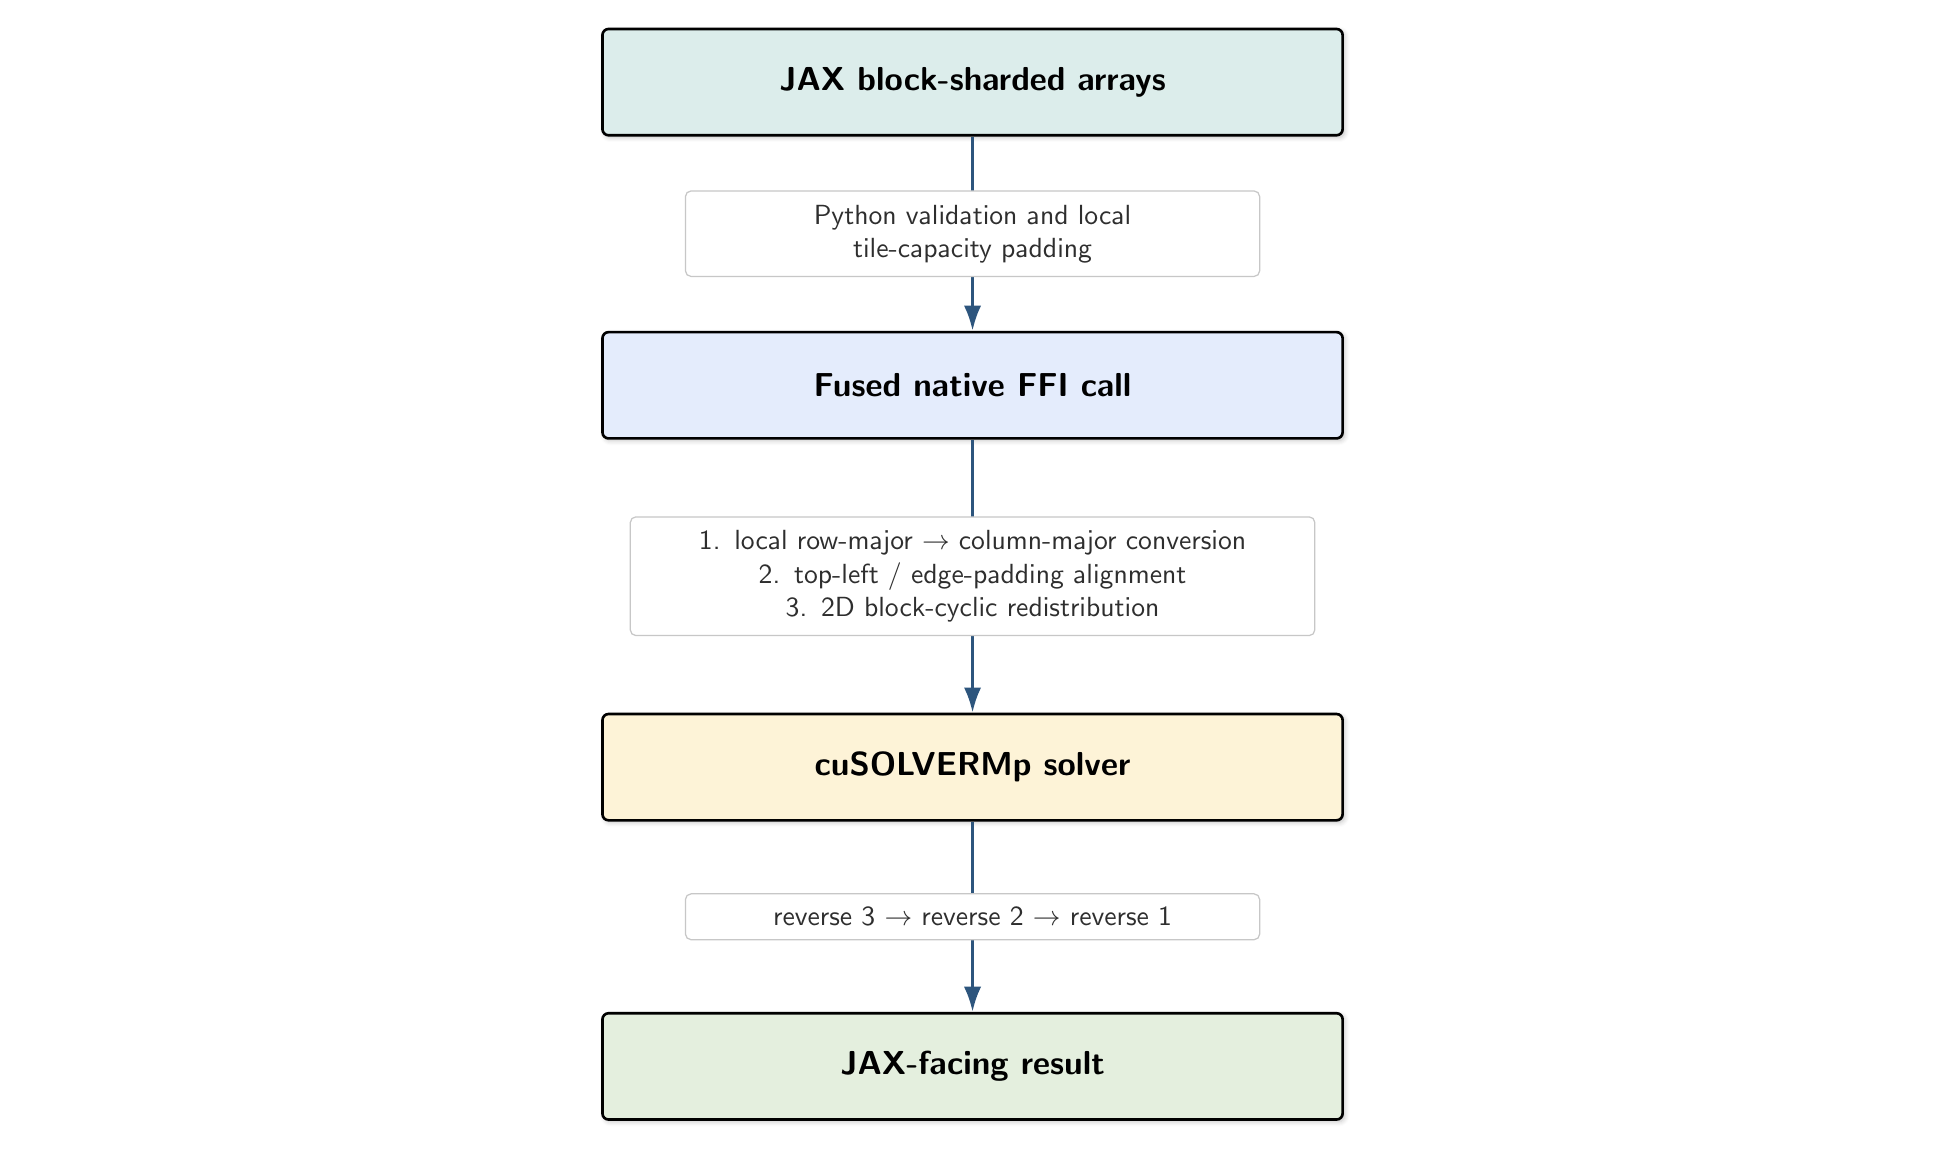
\begin{tikzpicture}[x=1cm,y=1cm]
  \path[] (-12cm,7cm) -- (12cm,7cm);
  \node[jax]    (jax1)    at (0,13.55) {JAX block-sharded arrays};
  \node[ffi]    (ffi1)    at (0,9.70)  {Fused native FFI call};
  \node[solver] (solver1) at (0,4.85)  {cuSOLVERMp solver};
  \node[result] (result1) at (0,1.05)  {JAX-facing result};

  \draw[flow] (jax1) --
    node[transition medium,midway]
      {Python validation and local\\tile-capacity padding}
    (ffi1);

  \draw[flow] (ffi1) --
    node[transition wide,midway]
      {1. local row-major $\rightarrow$ column-major conversion\\
       2. top-left / edge-padding alignment\\
       3. 2D block-cyclic redistribution}
    (solver1);

  \draw[flow] (solver1) --
    node[transition medium,midway]
      {reverse 3 $\rightarrow$ reverse 2 $\rightarrow$ reverse 1}
    (result1);
\end{tikzpicture}

\end{document}
